\subsection{Logical View}
\label{sec:logicalview}

The architecture is based around a reusable application logic layer, that connects to the
local file system and a database as needed. Additionally, it can easily be used by
both the Web-Only UI and the Local UI.

\begin{figure}[htb]
	\centering
	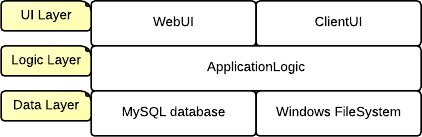
\includegraphics[width=0.7\textwidth]{Software_architecture/graphics/application-layers.png}
	\caption{Layers of the application}
	\label{fig:application-layers}
\end{figure}

Because of this structure, we have an architecture that is split in that it supports two
parallel UI layers and two parallel data layers (see Figure \ref{fig:application-layers}).

From these layers our package diagram almost directly follows (Figure \ref{fig:package-diagram}):
To communicate with the different data layers, we have two separate models. It is important to
note that the \emph{LocalFileModel} connects to both the file system (in most situations) and
to the database (when this is explicitly requested).

In using the Model-View-Controller pattern to separate to visuals (WebUI, ClientUI) from the
data behind (LocalFileModel, WebFileModel) by communicating through the Controller, we achieve
low coupling and high cohesion. We focus on extensibility and easy replacement of different
parts without it affecting other parts of the software. This is useful in a proof-of-concept as
more sturdy, production-level classes should be put in place before the system is distributed.

\begin{figure}[htb]
	\centering
	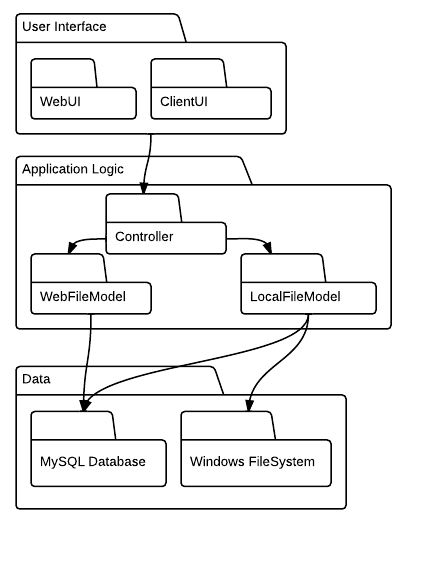
\includegraphics[width=0.7\textwidth]{Software_architecture/graphics/package-diagram.png}
	\caption{Package Diagram showing dependencies from the UIs to the Application Logic}
	\label{fig:package-diagram}
\end{figure}

The Controller additionally depends on a UserModel being present. This model handles verification
and creation of user accounts.

With the overall architecture in place, the last important logical component of the architecural design
consists of the basic classes that all packages use (Figure \ref{fig:basic-classes}): \emph{Document},
\emph{Folder} and \emph{Project}. These are mostly defined in their implementations of \emph{IItemContainer}
and \emph{IItem}. \emph{IItem} defines an "item"; something that can be contained in an
\emph{IItemContainer}. This is important as Folders may both \emph{contain} and \emph{be contained},
whereas Documents may only be contained and Projects may only contain.

This structure, with its use of \emph{composition} (in that folders may contain folders), results in a
dynamically extensible hierachy, much like the one found in most filesystems. An additional constraint
in the architecture is that a root element will {\bf always} be a project, and as such it is easy to
manage bundles of files by their parent project.

\begin{figure}[htb]
	\centering
	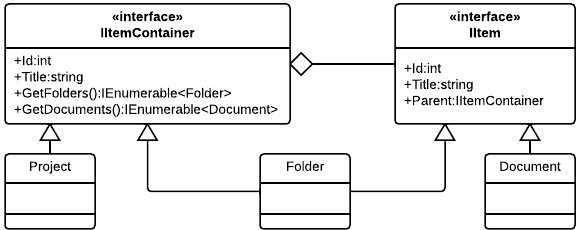
\includegraphics[width=0.9\textwidth]{Software_architecture/graphics/basic-classes.png}
	\caption{Basic classes sent around in the application and their relative relationship.}
	\label{fig:basic-classes}
\end{figure}